\documentclass[12pt]{article}
\usepackage{amsmath}
\usepackage[space]{cite}
\usepackage{enumitem}
\usepackage{float}
\usepackage{graphicx}
\graphicspath{ {./images/} }
\restylefloat{table}
\usepackage{makecell}

% this list puts numbers in parentheses
\newlist{nicelist}{enumerate}{1}%
\setlist[nicelist]{label={(\arabic*)}}%

% these commands make for nicer-looking tables
\renewcommand\theadalign{bc}
\renewcommand\theadfont{\bfseries}


\begin{document}

\begin{abstract}
	Silver carp (\emph{Hypophthalmychthys molitrix}) are one of four primary species of invasive cyprinids in the Mississippi River Basin. They threaten the ecosystems in which they have been introduced by competing with native planktivores and the early life stages of other native fishes. Additionally, silver carp can injure recreational boaters, thus causing negative economic impacts. To mitigate their spread, non-physical barriers such as electrical barriers, bubble curtains, carbon dioxide, and acoustic deterrents have been installed at locks and dams throughout the Mississippi River Basin. In this article, we focus on acoustic deterrents, and investigate their effect on behavioral changes on silver carp, using data from a 2018 pond study performed at the Columbia Environmental Research Center. We use a modeling approach combining continuous-time correlated random walks with a hidden Markov model for two behavioral states. We incorporate interpolated sound-intensity values from the acoustic deterrent as a novel covariate. We also investigate the effect of pond-surface temperature and diel effects on silver carp behavior changes.
\end{abstract}

\title{Modeling Behavioral Changes of Invasive Carp in Response to Acoustic Deterrents}
\author{
	Reichenbach, Matthew \\
	\texttt{matthew.p.reichenbach@usace.army.mil}
	\and
	Sava, Elena \\
	\texttt{Elena.Sava@usace.army.mil}
	\and
	Maloney, Megan \\
	\texttt{Megan.C.Maloney@usace.army.mil}
	\and
	Woodley, Christa \\
	\texttt{Christa.M.Woodley@usace.army.mil}
	\and
	Urbanczyk, Aaron \\
	\texttt{Aaron.C.Urbanczyk@usace.army.mil}
}
\date{\today}

\maketitle

\section{Introduction}

	\subsection{Invasive Carp in the Mississippi River Basin}

	Silver carp (\emph{Hypophthalmychthys molitrix}) were introduced into North America in the 1960s and 1970s, and have since become invasive in the Mississippi River Basin. Due to their large population increase \cite{DeBoer2018}, these large-bodied planktivores threaten aquatic ecosystems \cite{Kolar2007, Pegg2002, Sullivan2018} by competing for resources with native planktivores, and with the early life stages of other native fishes \cite{Solomon2016, Phelps2017, Fritts2018}.  Additionally, silver carp can cause injure fisherman and recreational boaters, which can have significant economic impacts \cite{Solomon2016, Chick2020}.

	\subsection{Deterrent Systems}

	To mitigate the economic and environmental impacts of the silver carp, researchers and wildlife managers have developed a number of tools to reduce their population, from marketing them for human consumption (Morgan2018) to the development of novel gears techniques (Collins2015, Butler2019, Ridgeway2020, Chapman2020). Given their wide dispersal throughout the Mississippi River Basin (USFWS2017), researchers have also developed tools to manage the dispersal of silver carp; these include non-physical deterrents like electrical barriers (Clarkson2004), bubble curtains (Zielinski2016), carbon dioxide (Donaldson2016, Cupp2021), and acoustic deterrents (Vetter2015, 2017), and combinations of these (Ruebush2012, Dennis2019). To increase their effectiveness at deterring dispersal and migration, these deterrents have been installed at key pinch-points along the Mississippi River system  where fish passage controlled (for example, a navigation lock (ACRCC2018)).
	
	The electric barrier installed in the Chicago Area Waterways System (CAWS) has significantly mitigated the upstream movement of silver carp (Parker2016). However, electrical deterrents are not species-specific (Reynolds1996, Dolan2003), and thus can impede the migratory behavior of native species. In addition to these spillover ecological effects, electrical deterrents are unsuited to places which humans frequent for recreation and navigation, due to the danger which they pose.
	
	Acoustic deterrents offer the possibility of selectively targeting silver carp, while posing less risk to humans. A number of studies have shown that a broad-frequency $100$hp outboard motor sound repeatedly deterred silver carp, but were not deterred by pure tones (Vetter2015, 2017, Murchy2017). Additionally, Dennis2019 found that a $40$hp sound, and a proprietary sound, deterred bigheaded carp (which silver carp belong to) as they attempted to pass through a flume. In both of these cases, the carps stopped responding to the deterrent by the end of the study, suggesting habituation or fatigue.
	
	These studies indicate that multi-frequency acoustic signals may deter silver carp, but their effectiveness under a more natural setting remains unknown. These boat-motor sounds also come with energetic demands and subsequent wear on the sound projectors which more compatible signals could lessen. To this end, we study the response of silver carp in a pond study to three acoustic stimuli: a $100$hp outboard motor sound, as in (Vetter2015, 2017, Murchy2017), along with two engineered sounds, which we denote Saw and Square. In addition to studying the response of carp at the onset of the acoustic stimulus, we also study changes to their response over a 72-hour period. We hypothesized that silver carp would exhibit changes to their behavioral state at the onset of the stimulus, but with less marked response over the course of the 72-hour period.

	\subsection{Movement Modeling}
	
	In the last two decades, methods to collect highly detailed data on animal movements have become easily accessible \cite{McConnell2010, Tomkiewicz2010}. This has led to rapid development in state-space models of animal behavior, and of tools to allow non-specialists to implement the models \cite{Johnson2008, McClintock2012, Michelot2016, Whoriskey2017, McClintock2018}.
	
	We used hidden Markov models to study the effect of environmental covariates on carp behavior; we were primarily interested in the effects of sound type ($100$hp boat-motor or the engineered signals) and sound intensity on carp behavior. There has been limited research on this topic, but one recent paper (Faulkner et al, unpublished) found that sound-types were associated with changes to the behavioral states of carp. However, the authors did not incorporate a sound intensity covariate.
	
	We performed the data-processing and modeling in \texttt{R} \cite{Rlang2022}, primarily using the \texttt{momentuHMM} package \cite{McClintock2018} for location estimation and model fitting. We note that momentuHMM relies heavily on the \texttt{crawl} \cite{crawl} and \texttt{moveHMM} \cite{Michelot2016} packages.

\section{2018 CERC Pond Study} \label{sec:pond_study}

	The study consisted of five trials, each lasting 72 hours. For each of the five trials, one of four acoustic deterrent treatments (Control, 100hp, Saw, and Square) was assigned to four ponds. The experimental design and trial durations are included in Table \ref{tbl:pond_study}.
	
	\begin{table}[H]
	\centering
	\begin{tabular}{|c|c|c|c|c|}
		\hline
		\, & \thead{Pond 26} & \thead{Pond 27} & \thead{Pond 30} & \thead{Pond 31} \\
		\hline
		\makecell{\thead{Trial 1 \\ 6/11 to 6/14}} & Control & Square & 100hp & Saw \\
		\hline
		\makecell{\thead{Trial 2 \\ 6/26 to 6/29}} & Square & 100hp & Saw & Control \\
		\hline
		\makecell{\thead{Trial 3 \\ 7/10 to 7/13}} & 100hp & Saw & Control & Square \\
		\hline
		\makecell{\thead{Trial 4 \\ 7/24 to 7/27}} & Saw & Control & Square & 100hp\\
		\hline
		\makecell{\thead{Trial 5 \\ 8/07 to 8/10}} & Control &100hp & Saw & Square \\
		\hline
	\end{tabular}
	\caption{Locations of acoustic deterrent treatments during each trial.}
	\label{tbl:pond_study}
	\end{table}
	
	For each trial, each pond contained 20 silver carp, ten of whom had an acoustic telemetry tag which allowed us to gather large time series datasets of their locations. All fish were removed between trials, and new fish were placed in each pond.
	
	Over the course of each trial, an underwater speaker played the acoustic deterrent sample on a loop for 30 minutes; this process was repeated once every 3 hours. In this paper, we refer to each time the deterrent turns on as a \emph{repetition}. There were 24 deterrent repetitions per trial, for a total of 120 over the course of the study.

\section{Modeling Framework}

	In this study, we use a state-space model developed in \cite{Johnson2008, McClintock2012, Michelot2016, Whoriskey2017, McClintock2018}, which uses a continuous-time correlated random-walk (CTCRW) model to predict carp locations at regular timesteps, followed by a hidden Markov model (HMM) to infer behavioral states as a function of environmental covariates. We fit models over three blocks of time: 1 minute, 5 minutes, and 30 minutes after the acoustic deterrent turned on.
	
	 We used the R package \texttt{momentuHMM} \cite{McClintock2018} to fit the models, and performed spatial interpolations of sound intensity values with the kriging utilities in the \texttt{automap} package  \cite{Hiemstra2008}.

	\subsection{Continuous-time Correlated Random Walk (CTCRW)}
	
		In our pond study (see Section \ref{sec:pond_study}), the telemetry data has an irregular timestep; however, hidden Markov models require a constant timestep. To ensure this, we first fit a CTCRW model to the telemetry data, and used it to predict fish locations at a regular time step. To do this, we used the \texttt{crawlWrap} functions from the \texttt{momentuHMM} package \cite{McClintock2018}. This function is itself a wrapper of the \texttt{crwMLE} and \texttt{crwPredict} functions from the \texttt{crawl} package \cite{crawl}.
		
		The \texttt{crwMLE} function uses a Kalman filter to fit a continuous-time Ornstein-Uhlenbeck velocity process for each fish track, which is then integrated to form a location process. That is, for a given time-separation $\Delta$, the velocity $\nu_c(t)$ in the direction $c \in \{1, 2\}$ is modeled by the autoregressive equation
		\begin{align}
			\nu_c(t + \Delta) := \gamma_c + e^{-\beta \Delta} (\nu_c(t) - \gamma_c) + \zeta_c(\Delta). \label{eqn:velocity}
		\end{align}
		Here, $\gamma_c$ is a mean-velocity parameter, $\beta$ is an autocorrelation parameter, and $\zeta_c(\Delta)$is a normal random variable with zero mean, and variance which grows with $\Delta$. Putting $\vec \nu(t) := [\nu_1(t), \nu_2(t)]^T$, and assuming that the velocity processes in each coordinate are independent, the continuous-time location process is given by
		\begin{align}
			\vec \mu(t) := \mu(0) + \int_0^t \vec \nu(u) \, du. \label{eqn:position}
		\end{align}
		In order to use the Kalman filter to estimate parameters, one can reformulate the processes (\ref{eqn:velocity}) and (\ref{eqn:position}) as a Gaussian linear state-space model for a univariate observation; the details are included in \cite{Johnson2008}.
		
		Using the fitted-model output of \texttt{crwMLE}, the function \texttt{crwPredict} then predicts locations at the specified timesteps \cite{crawl, Johnson2008}. For the 1-minute and 5-minute models, we used a timestep of 2 seconds, which is close to the average timestep in the telemetry data. For the 30-minute models, a 2 second timestep was too frequent to allow model-fitting in a reasonable amount of time; instead, we opted to for a 6-second interval in the 30-minute models.

	\subsection{Hidden Markov Models (HMMs)}
	
		HMMs are particularly well-suited to studying the behavioral changes of fish in response to environmental stimuli, because they attempt to identify hidden ``states" given observed data \cite{Rabiner1989}. We assume that the fish exhibit two behavioral states, which we denote ``exploratory" and ``encamped"; the former is characterized by directed motion at a greater speed, and the latter is characterized by random (uniform) motion at slower speeds. These two states describe motion in many species, such as elk \cite{Morales2004, Fryxell2008}, gray brocket deer \cite{Grotta-Neto2019}, elephants \cite{Roever2014, Vogel2019}, and grey seals \cite{Breed2009}. Though these are mammalian examples, with only one aquatic species, a visual inspection of the carp telemetry data indicates that individuals do exhibit encamped and exploratory behaviors as well.
		
		We fit HMMs using the \texttt{fitHMM} function from the \texttt{momentuHMM} package. These models consist of probability distributions for step lengths and turning angle for each state, and a state transition matrix. In general, HMMs may consist of an arbitrary number of states $n$, but we investigated the case when $n = 2$. We modeled the step lengths as as Gamma distributions, and the turning angles as von Mises distributions.
	
	\subsection{Covariates}
	
		We explored the effect of five covariates on carp behavior, \emph{Trial, Treatment, Diel, Temperature, and Intensity}, by modeling the step length means and state transition probabilities as linear functions of the covariates. We only included Diel as a covariate in model formulas when sunrise and sunset occur during the same sound repetition. For the sound repetitions in which that occurs, we fit a total of 32 models, and for the sound repetitions in which a sunrise or sunset does not occur, we fit 16 models. These values come from the fact that
		\[2^n = \sum_{i=0}^n {n \choose i},\]
		where $i$ is the number of covariates to include in a formula. For the sound repetitions which contain a sunrise or sunset, we use all five covariates, so $n = 5$ covariates. Otherwise, we ignore the formulas with Diel, in which case $n = 4$. Also, we take $i = 0$ to be the intercept-only formula $\sim$1.
		
		The parameters of the HMMs which we modeled as linear functions of the covariates were the mean step lengths, $\mu_1$ and $\mu_2$; the mean turning angles, $\theta_1$ and $\theta_2$, and the statetransition probabilities $\lambda_{1 \to 2}$ and $\lambda_{2 \to 1}$. Here, $\mu_i$ and $\theta_i$ are the mean step length and turning angle, respectively, for behavioral state $i = 1, 2$, and $\lambda_{i, j}$ denotes the probability that an individual switches from state $i$ to state $j$ during the time step, which were modeled as multinomial logit functions \cite{Michelot2016}. We used the intercept-only formula $\sim$1 to model the shape parameters of the Gamma and von Mises distributions in each HMM.
		
		\subsubsection{Factor Covariates}
		
			The \emph{Trial} covariate has five levels which correspond to the trial in the study: 1, 2, 3, 4, and 5. The \emph{Treatment} covariate has four levels which correspond to the type of acoustic deterrent played in the ponds, namely Control, 100hp, Saw, and Square. Details of the \emph{Trial} and \emph{Treatment} are included in Table \ref{tbl:pond_study}.
			
			The \emph{Diel} covariate has two levels, Day and Night. We defined Day to mean that a data point occurred after local sunrise and before local sunset on the same day, and Night to mean that a data point occurred after local sunset and before local sunrise on the following day. We only fit models with formulas including the Diel covariate when sunrise or sunset occurred within the particular dataset. This never occurs in the 1 minute datasets, only in Repetitions 1 \& 9 for the 5 minute datasets, and Repetitions 1, 9, \& 17 in the 30 minute datasets.
		
		\subsubsection{Numerical Covariates} \label{sec:num-cov}
		
			Pond surface temperature was recorded throughout the study, at 15 minute intervals in each pond. However, our predicted location data has a much finer temporal resolution: 2 seconds for the two short-term datasets (1 minute and 5 minutes after the sound stimulus), and 6 seconds for the long-term dataset (30 minutes after the sound stimulus). We incorporated temperature values into these datasets by performing a linear interpolation between each recorded value. Figure \ref{img:temperature} shows the temperature recordings in each pond over the course of each trial.
			
			\begin{figure}
				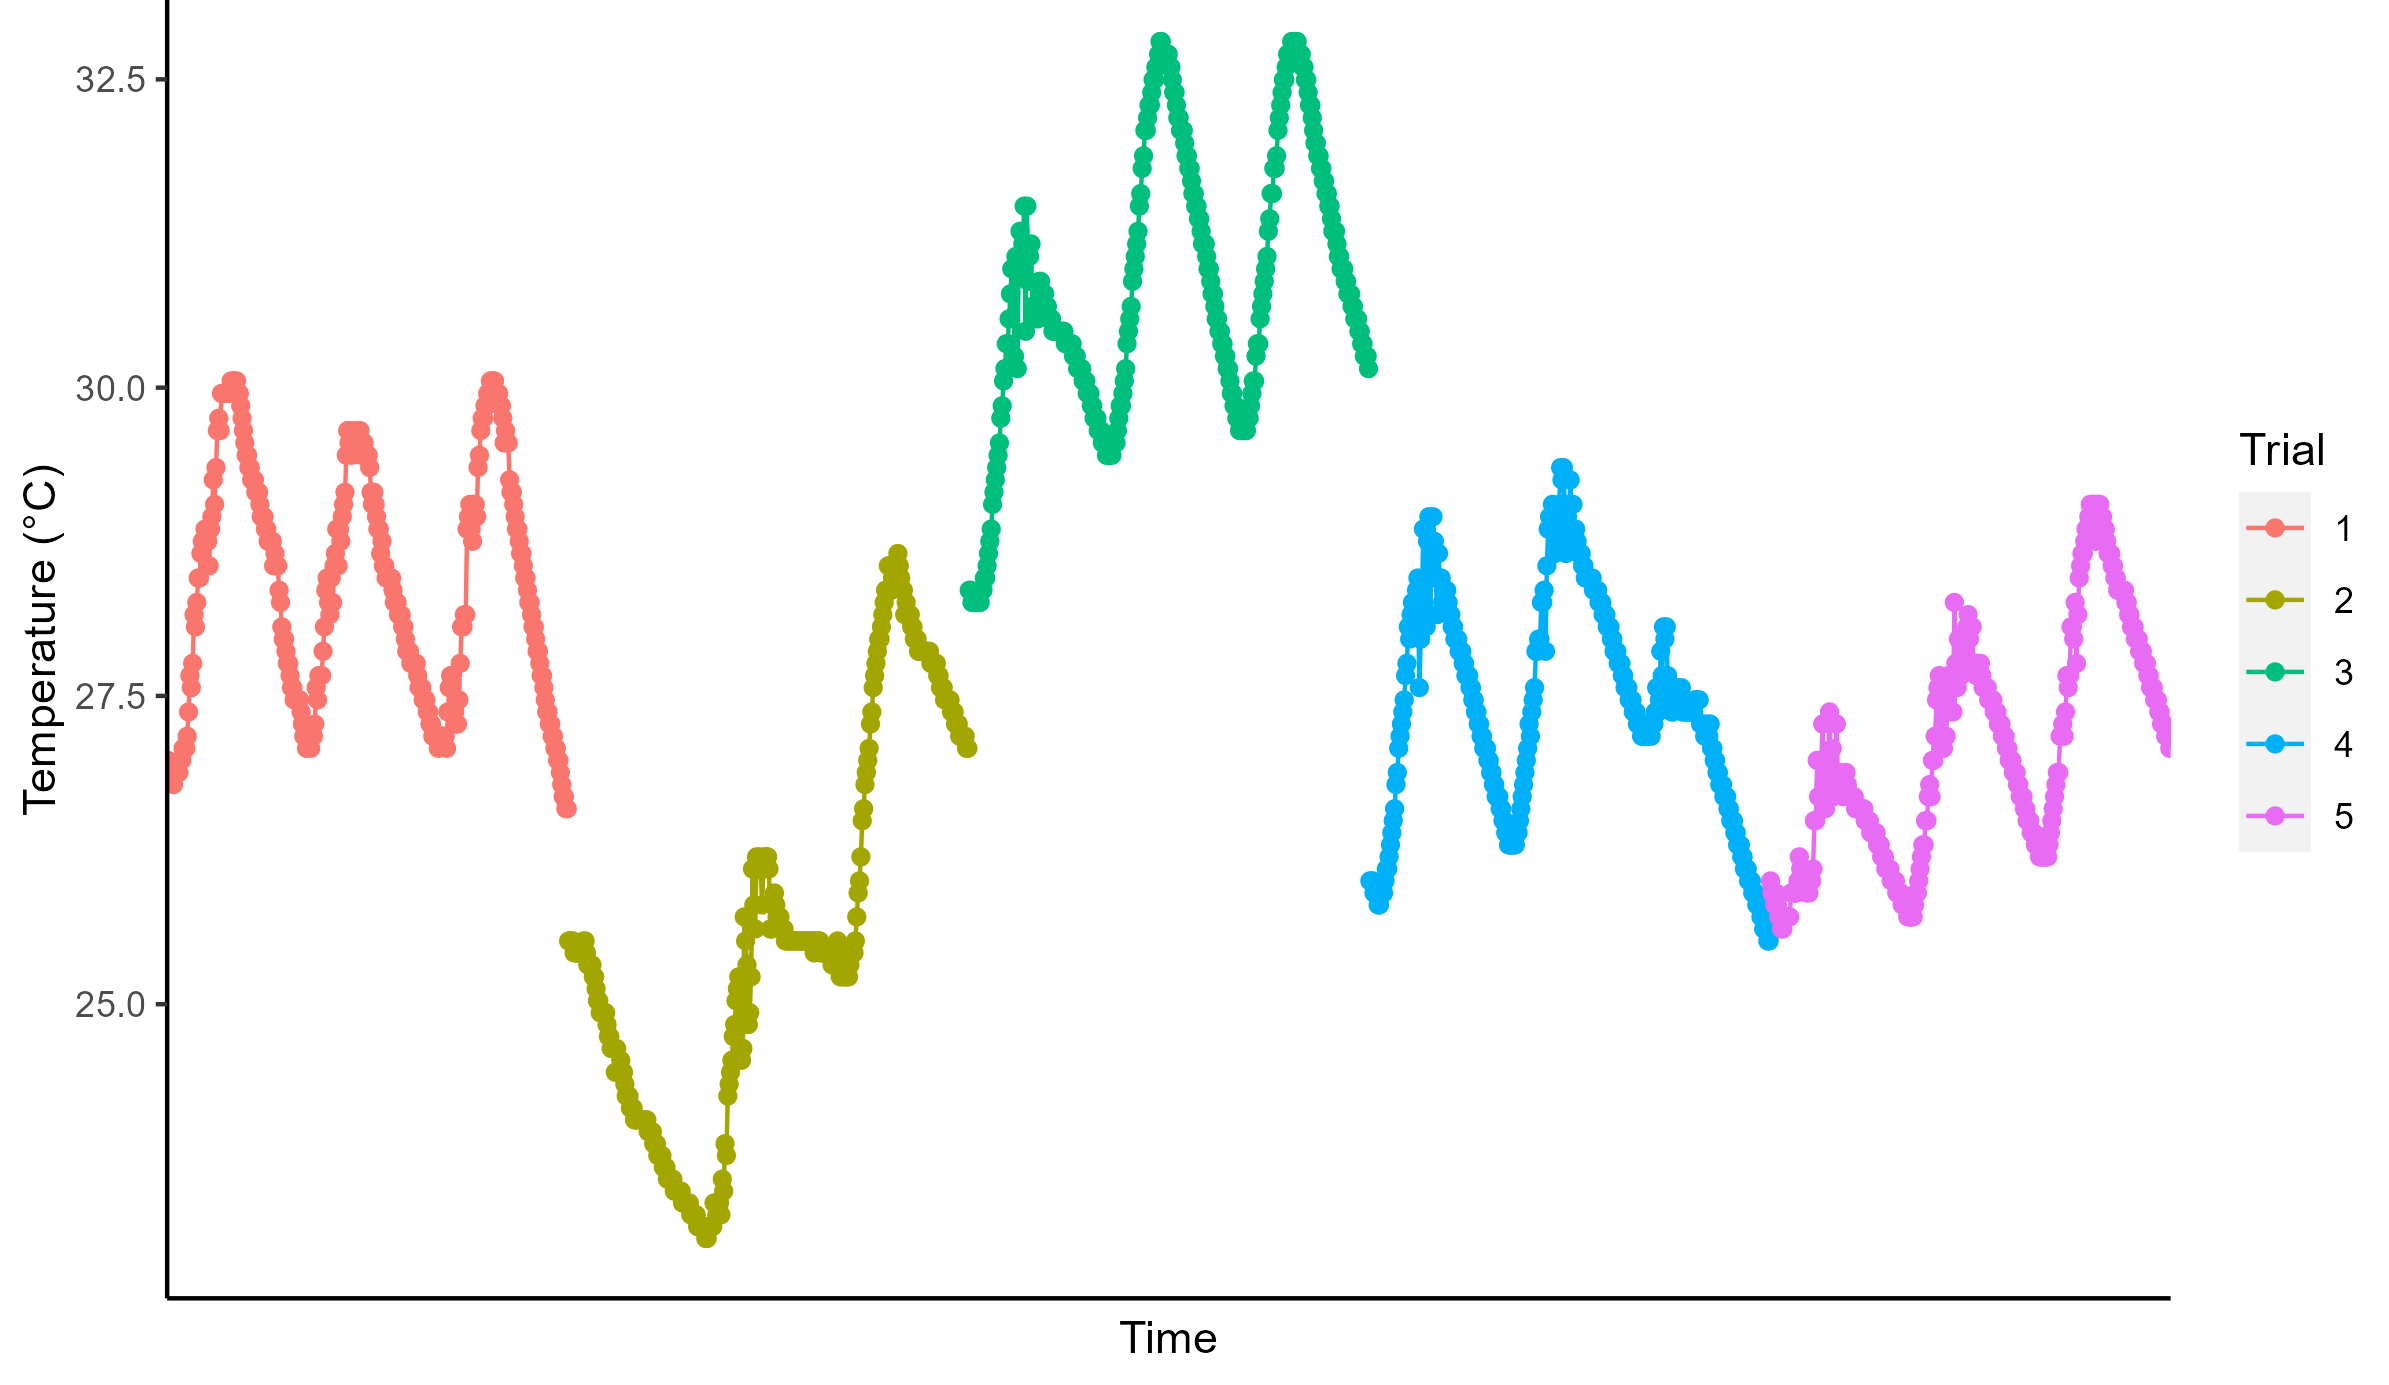
\includegraphics[width=\textwidth]{pond_26_temp.png}
				\caption{Temperature readings for Pond 26 throughout the 2018 CERC study.}
				\label{img:temperature}
			\end{figure}
		
			In order to incorporate the sound intensity as a covariate in the predicted tracks, we used the spatial interpolation method known as \emph{kriging} from the R package \texttt{automap} \cite{Hiemstra2008}. Kriging is especially useful when interpolated values are assumed to have some spatial autocorrelation, like acoustic signal intensities in water will. Kriging has the benefit of being an ``exact interpolator", meaning that the value predicted for any observed location will equal the observed value. Additionally, the interpolated values from the kriging process will be the best linear unbiased predictors.
			
			The kriging involves two steps: fitting a model to the variogram plot, then using this model to find weights which are used to interpolate missing values. The variogram plots half the mean-squared difference between the values at all pairs of points, against the distance between each pair. The \texttt{automap::autoKrige} function automatically determines which model fits the variogram best, by comparing fits of spherical, exponential, Gaussian, and a model from the Matern family of functions \cite{Hiemstra2008}. 
			
			Using whichever models fits the variogram best, the weights $w_i = w_i(x_0)$ can be calculated for each any unobserved point $x_0$, and the interpolated value $\hat z(x_0)$ is then a linear combination of these weights with the observed values $z(x_i)$, for $i = 1, \ldots, n$:
			
			\begin{align*}
				\hat z(x_0) &= \begin{bmatrix} w_1 & w_2 & \cdots & w_n \end{bmatrix} \begin{bmatrix} z(x_1) \\ z(x_2) \\ \vdots \\ z(x_n) \end{bmatrix} \\
				&= \sum_{i = 1}^n w_i(x_0) z(x_i)
			\end{align*}
			
			Further details on how the weights $w_i(x_0)$ at a given point can be computed are given in CITE A BOOK HERE.
			
			For our purposes, sound intensity readings (dB re 1 $\mu$Pa) were recorded once before the trials began, at 98 locations in each pond, and for each sound treatment except the Control. We used these values, along with an automatic kriging process, to interpolate sound intensity values which we incorporated into the movement tracks in each pond. Although there were 24 sound repetitions during the study study, intensity readings were not taken each time the sound turned on. Hence, we assumed that the readings taken before the the trials began were representative of the readings during each repetition. In order to incorporate reasonable values for sound intensity in the Control ponds, we sampled from a Gaussian random variable with parameters given in \cite{Wysocki2007} for a concrete pond.
			
			Figure \ref{img:intensities} shows interpolated sound intensity values in each pond from the kriging process.
			
			\begin{figure}[H]
				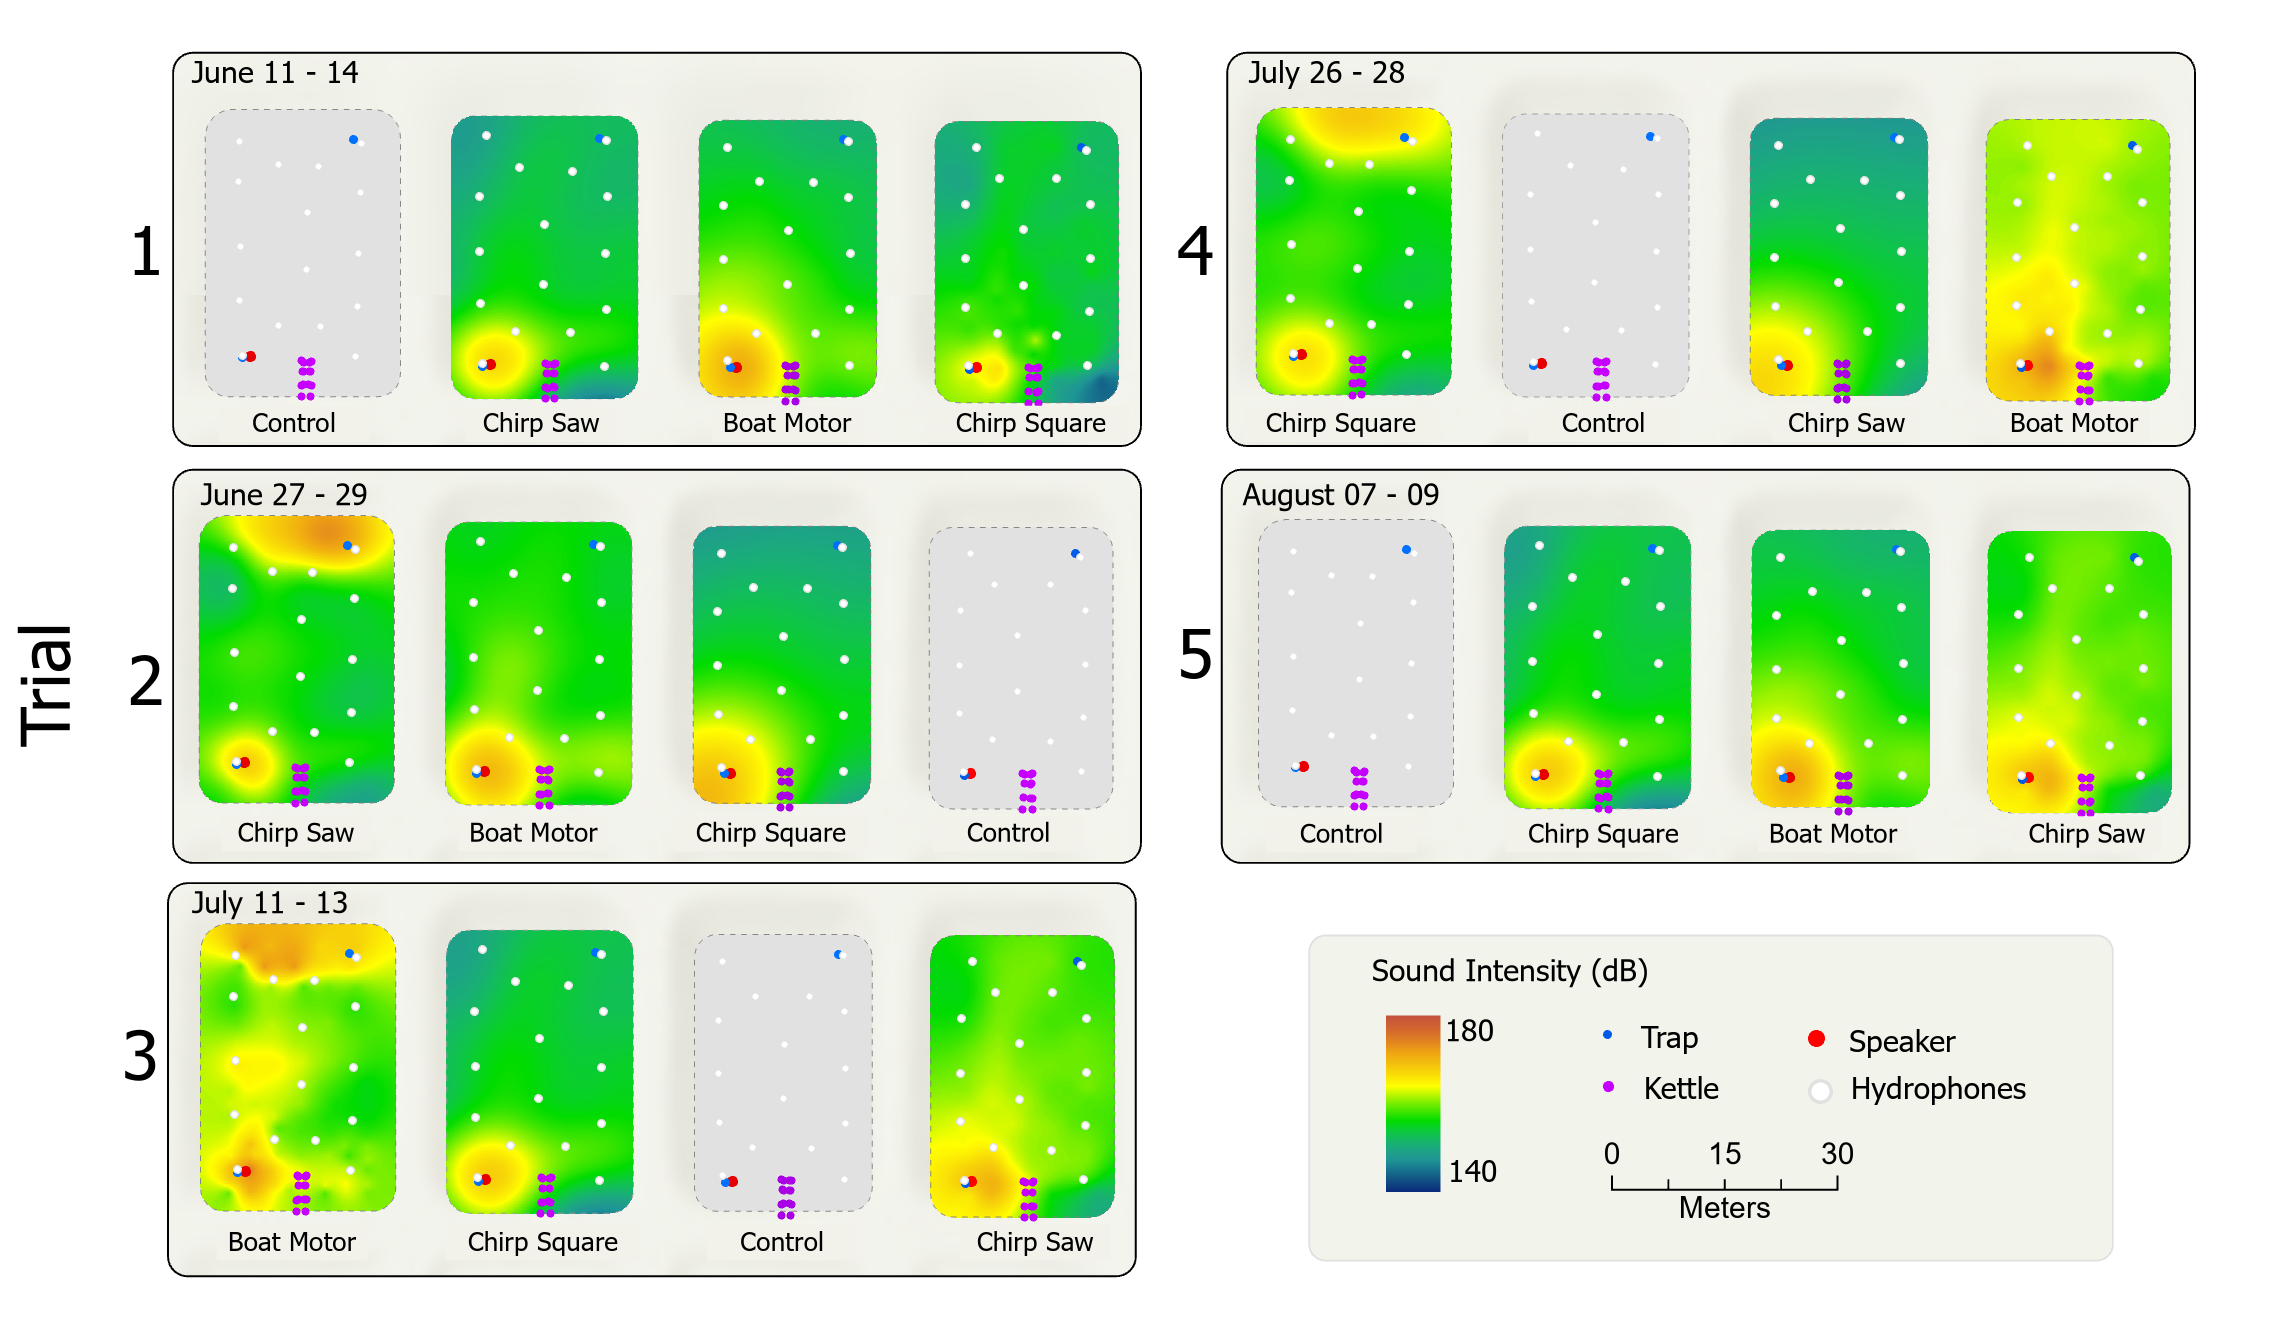
\includegraphics[width=\textwidth]{intensities.png}
				\caption{Interpolated sound intensity values from the kriging process.}
				\label{img:intensities}
			\end{figure}		

\section{Results}

	\subsection{Top Models by AIC Score}
	
		In order to determine whether sound intensity was a good predictor of carp behavior, we first determined the frequency of the \emph{dB} covariate among the top model formulas for the 24 repetitions. For each sound repetition, and for each time-interval (1 minute, 5 minute, and 30 minutes after the sound exposure), we determined the top model according to Akaike's Information Criterion, or AIC score. Table \ref{tbl:aic_scores} records the formulas of these top models; to simplify notation, we write \emph{dB}, \emph{Trt}, and \emph{Temp} in place of \emph{Intensity, Treatment, and Temperature}, respectively.
		
			\begin{table}[H]
			\centering
			\begin{tabular}{|c|c|c|c|}
				\hline
				\thead{Repetition} & \thead{1 min.} & \thead{5 min.} & \thead{30 min.} \\
				\hline
				1 & $\sim$Trial+Temp+Trt & $\sim$Trial+Temp+Diel+Trt & $\sim$Trial+Trt \\
				\hline
				2 & $\sim$Trial+Trt & $\sim$Trial+Temp+Trt & $\sim$Trial+Temp+Trt \\
				\hline
				3 & $\sim$Trial+Trt & $\sim$Trial+Temp+Trt & $\sim$Trial+Temp+Trt \\
				\hline
				4 & $\sim$Trial+dB+Trt & $\sim$Trial+dB+Trt & $\sim$Trial+Trt \\
				\hline
				5 & $\sim$Trial+Trt & $\sim$Trial+Trt & $\sim$Trial+Temp+Trt \\
				\hline
				6 & $\sim$Trial+dB+Trt & $\sim$Trial+Trt & $\sim$Trial+Trt \\
				\hline
				7 & $\sim$Trial+Temp+dB & $\sim$Trial+Temp+Trt & $\sim$Trial+Temp+Trt \\
				\hline
				8 & $\sim$Trial+Trt & $\sim$Trial+Trt & $\sim$Trial+Temp+Trt \\
				\hline
				9 & $\sim$Trial+Temp+Trt & $\sim$Trial+dB+Trt & Trial+Trt \\
				\hline
				10 & $\sim$Trt & $\sim$Trial+Temp+Trt & $\sim$Trial+Temp+Trt \\
				\hline
				11 & $\sim$Trial+Trt & $\sim$Trial+Trt & $\sim$Trial+Temp+Trt \\
				\hline
				12 & $\sim$Trial+dB+Trt & $\sim$Trial+Temp+Trt & $\sim$Trial+Temp+Trt \\
				\hline
				13 & $\sim$Trial & $\sim$Trial+Temp+Trt & $\sim$Trial+Temp+Trt \\
				\hline
				14 & $\sim$Trial+Trt & $\sim$Trial+Trt & $\sim$Trial+Temp+dB+Trt \\
				\hline
				15 & $\sim$Trial+Temp+Trt & $\sim$Trial+Trt & $\sim$Trial+dB+Trt \\
				\hline
				16 & $\sim$Trial+Trt & $\sim$Trial+Trt & $\sim$Trial+Trt \\
				\hline
				17 & $\sim$Trial+Trt & $\sim$Trial+Trt & $\sim$Trial+Temp+Trt \\
				\hline
				18 & $\sim$Trial+Trt & $\sim$Trial+Trt & $\sim$Trial+Temp+Trt \\
				\hline
				19 & $\sim$Trial+Temp+Trt & $\sim$Trial+Trt & $\sim$Trial+Trt \\
				\hline
				20 & $\sim$Trial+Trt & $\sim$Trial+Temp+Trt & $\sim$Trial+Temp+Trt \\
				\hline
				21 & $\sim$Trial+Trt & $\sim$Trial+Trt & $\sim$Trial+Trt \\
				\hline
				22 & $\sim$Trial+Trt & $\sim$Trial+Temp+Trt & $\sim$Trial+Trt \\
				\hline
				23 & $\sim$Trial+Trt & Trial+Trt & $\sim$Trial+Trt \\
				\hline
				24 & $\sim$Trial & $\sim$Trial+Temp+Trt & Trial+Temp+Trt \\
				\hline
			\end{tabular}
			\caption{Formulas of top models by AIC score.}
			\label{tbl:aic_scores}
			\end{table}
	
		Given that only a few model formulas occur in the top models, the table in Figure \ref{tbl:aic_scores} is summarized in the formula frequency table in Figure \ref{tbl:frm_freq}:
		
			\begin{table}[H]
				\centering
				\begin{tabular}{|c|c|c|c|c|}
					\hline
					\thead{Formula} & \makecell{\thead{1min \\ Frequency}} & \makecell{\thead{5min \\ Frequency}} & \makecell{\thead{30min \\ Frequency}} & \thead{Total} \\
					\hline
					$\sim$Trial+Trt & 13 & 12 & 9 & 34 \\
					\hline
					$\sim$Trial+Temp+Trt & 4 & 9 & 13 & 26 \\
					\hline
					$\sim$Trial+dB+Trt & 3 & 2 & 1 & 6 \\
					\hline
					$\sim$Trial & 2 & 0 & 0 & 2 \\
					\hline
					$\sim$Trial+Temp+dB & 1 & 0 & 0 & 1 \\
					\hline
					$\sim$Trt & 1 & 0 & 0 & 1 \\
					\hline
					$\sim$Trial+Temp+Diel+Trt & 0 & 1 & 0 & 1 \\
					\hline
					$\sim$Trial+Temp+dB+Trt & 0 & 0 & 1 & 1 \\
					\hline
				\end{tabular}
				\caption{Frequency of formulas in top models.}
				\label{tbl:frm_freq}
			\end{table}
			
	\subsection{State Transition Probabilities}
	
		To determine whether the covariate \emph{dB} had a common effect on carp behavior, we investigated plots of the state transition probabilities $\lambda_{i, j}$, with $i, j \in \{1, 2\}$, as a function of dB (re 1 $\mu$Pa). The probabilities $\lambda_{i, j}$ are modeled as multinomial logit functions, the details of which are given in \cite{Michelot2016}. These plots indicate how the probability of changing behavioral states is correlated with changes to dB levels in the pond. Recall that $\lambda_{i, j}$ gives the probability that an individual will be in behavioral state $j$ at time $n+1$, given that they are in behavioral state $i$ at time $n$. Also, since we only consider two behavioral states, we have the identities
		\begin{align*}
			\lambda_{1, 1} + \lambda_{1, 2} &= 1 \\
			\lambda_{2, 1} + \lambda_{2, 2} & = 1.
		\end{align*}
		
		When fitting models, we associated $i = 1$ to the \emph{exploratory} behavioral state, and $i = 2$ to the \emph{encamped} state.
		
		\subsubsection{1-Minute Models}
		
		\subsubsection{5-Minute Models}
		
		\subsubsection{30-Minute Models}

\section{Conclusion}

\bibliographystyle{apalike}
\bibliography{references}

\end{document}